\Chapter{Backend Dokumentáció}

Ebben a fejezetben azt fogom bemutatni, hogy egy Java (Spring Boot) applikáció hogyan épül fel.
\Section{Projekt inicializálás}

A projektet a Spring Boot Initializr segítségével hoztam létre.

\begin{figure}[h]
\centering
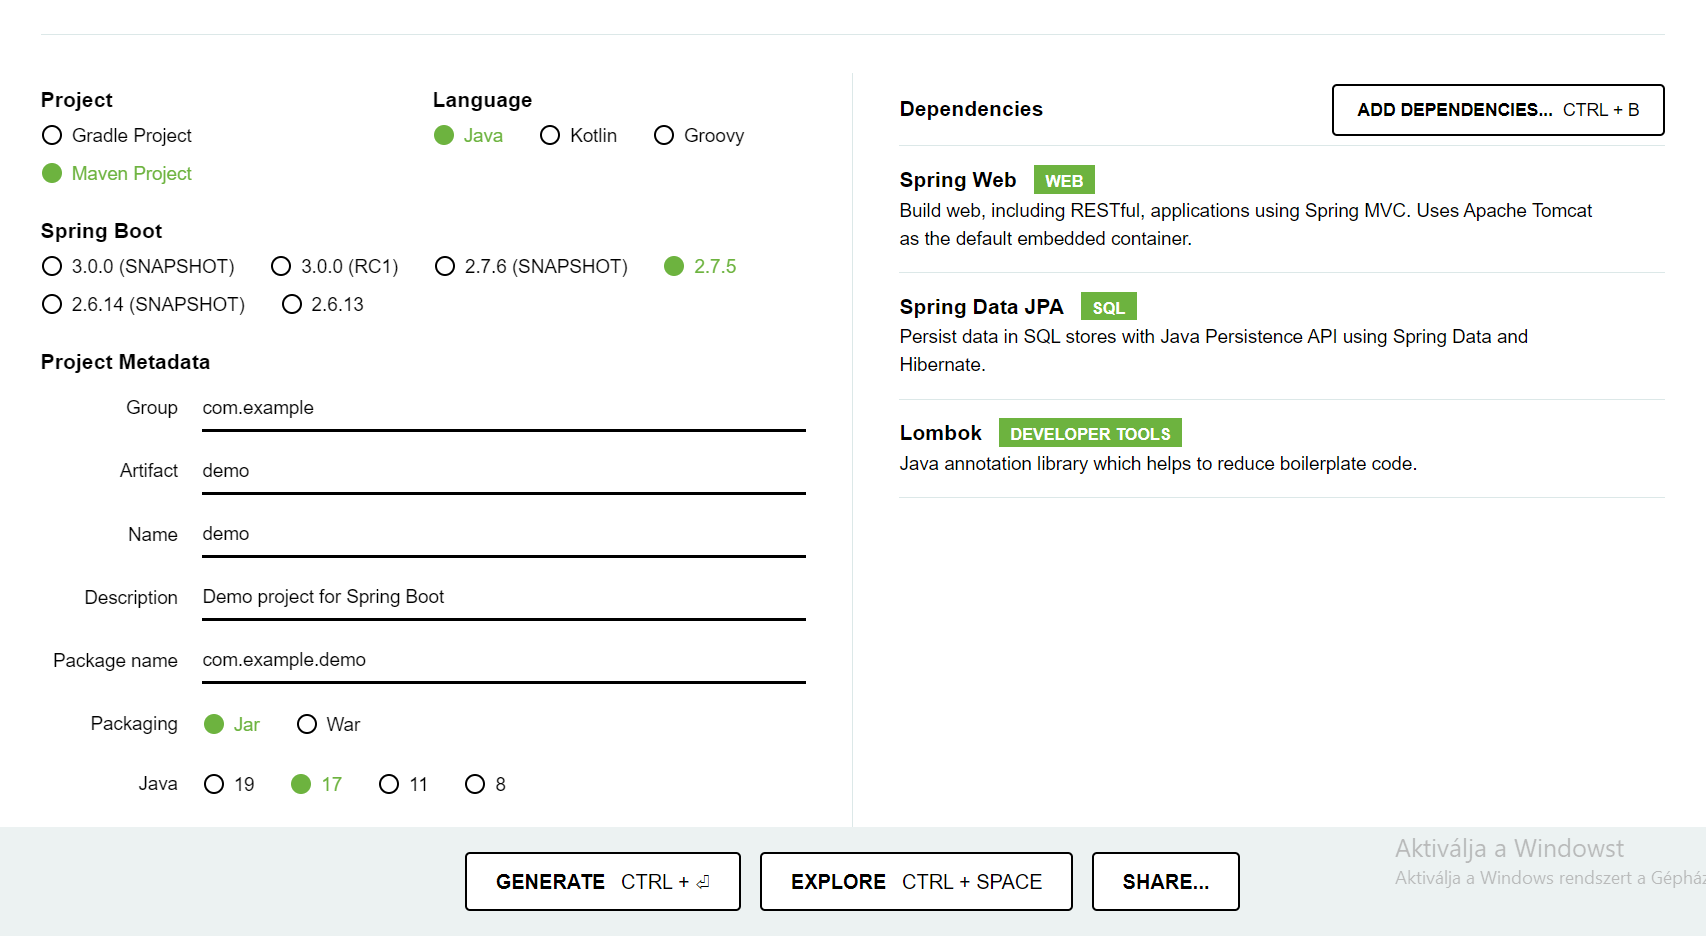
\includegraphics[scale=0.37]{images/Spring_init.png}
\caption{Spring Boot Initializr \cite{SpringInit}}
\label{fig:Spring_Boot_Initializr}
\end{figure}

Ahogy a \ref{fig:Spring_Boot_Initializr}. ábrán is látszik, ki lehet választani, hogy milyen típusú projekt legyen, milyen nyelven szeretnénk elkészíteni, a Spring Boot verzióját, metaadatokat, milyen Java verzióra szeretnénk fejleszteni.

Függőségeket tudunk megadni. A létrehozáskor a Spring Web-et, a Spring Data JPA-t és a Lombok-ot adtam hozzá.

A függőségek leírása a \textit{pom.xml} fájlban találhatóak meg. 

Mikor mindent kiválasztottunk a "GENERATE" gombra kattitnva le is generálja nekünk az alap projektet.
\newpage

Az elkészített projekt mappaszerkezete a \ref{fig:Intelij-mappaszerkezet}. ábrán látható.
\begin{figure}[h]
\centering
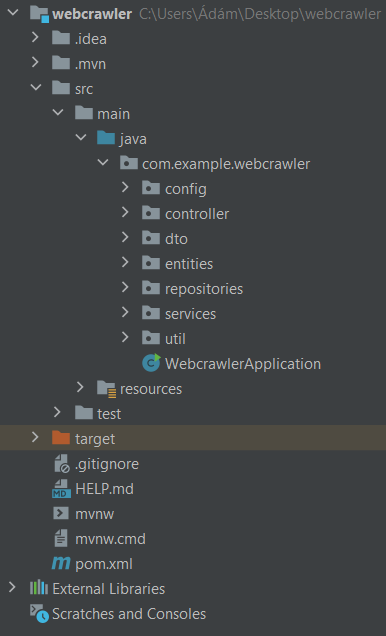
\includegraphics[scale=0.7]{images/Intelij-mappaszerkezet.png}
\caption{Intelij-mappaszerkezet}
\label{fig:Intelij-mappaszerkezet}
\end{figure}

Maga a szerver a \textit{http://localhost:8080/} címen fut.

\Section{Adatbázis létrehozása} 

Első lépésben az Adatbázis létrehozásához 2 függőséget kellett használnom, amit a \textit{pom.xml} fájlba kellett elhelyezni:
\begin{java}
<dependency>
	<groupId>org.springframework.boot</groupId>
	<artifactId>spring-boot-starter-data-jpa</artifactId>
</dependency>

<dependency>
	<groupId>org.postgresql</groupId>
	<artifactId>postgresql</artifactId>
	<scope>runtime</scope>
</dependency>
\end{java}

Miután a behelyezés megtörtént, az adatbázisunkat hozzá kell kapcsolni a szerve-
rünkhöz, ami az \textit{application.properties} fájlban történik. PostgreSQL-t adatbázist hasz-
nálok az adatok tárolására és a kapcsolat így jön létre a DB és a szerver között:

\begin{java}
spring.datasource.url=jdbc:postgresql://localhost:5432/cardb
spring.datasource.username=postgres
spring.datasource.password=Password
spring.jpa.properties.hibernate.dialect=
  org.hibernate.dialect.PostgreSQLDialect
spring.jpa.properties.hibernate.format_sql=true
\end{java}

Az URL az adatbázis szerver és maga az adatbázis eléréséhez szükséges. A szerver a 5432 porton fut és a cardb nevű adatbázisra lesz szükségünk.
A \textit{username} és \textit{password} ahhoz kell, hogy tudjuk magunkat hitelesíteni.

Következő lépésben létrehoztam a 3 adatbázis táblát (\textit{car}, \textit{search\_data}, \textit{users}) ami-
hez létrehoztam mindegyikhez egy \textit{entity}-t és egy \textit{repository}-t.

\textit{Entity}-n belül tudjuk megadni, hogy a táblán belül milyen oszlopok legyenek, és hogy mi legyen az elsődleges kulcs.

Példa egy \textit{Entity} Java osztályra, ami a \textit{users} nevű táblát hozza létre:

\begin{java}
@Getter
@Setter
@NoArgsConstructor
@AllArgsConstructor
@Entity
@Table(name="users")
public class User {
    @Id
    @GeneratedValue(strategy = GenerationType.IDENTITY)
    @Column(name = "user_id")
    private int id;

    @Column(name = "login")
    private String login;

    @Column(name = "password")
    private String password;

    @Column(name = "authority")
    private String authority;
}
\end{java}

A \textit{Repository}-ra azért van szükségünk, hogy a szerverünk tudjon kommunikálni az adatbázissal, tehát hogy tudjon adatot lekérdezni, felvinni törölni vagy éppen módosíta-
ni, és ehhez ki kell terjeszteni a \textit{JpaRepository} osztályt, ami tartalmaz alapvető művele-
teket.

Példa egy \textit{Repository} osztályra:

\begin{java}
@Repository
public interface UserRepository
extends JpaRepository<User, Integer> {
    List<User> deleteByLogin(String login);
    User findUserByLogin(String login);
}
\end{java}
\newpage

\Section{Autók importálása az adatbázisba}

Az adatok megszerzéséhez WebCrawlert \cite{WebCrawler} használok, ami azt jelenti, hogy az adato-
kat a weboldalak HTML-tartalmából gyűjtöm össze. Ehhez az egész weboldal felépítését át kell hozzá néznem, mivel tag-ek vagy éppen \textit{cssQuery}-vel lehet egyes adatokat kinyerni. 

Esetemben ez azért volt elég nehezen megoldható, mert arra is figyelni kellett, hogy vannak olyan autók a honlapon, amik nem rendelkeznek az összes adattal, ezért ki kellett szűrni az úgymond hibásan feltöltötteket. Olyan adatok hiányoztak sokszor, mint például: lóerő, hengerűrtartalom vagy éppen a futott kilométer nem volt megadva. Nagyjából az autóknak az 5\%-a volt hibás.

A lekérdezett adatok mennyisége attól függ, hogy hány oldalt fésülök át a Crawler segítségével, és hogy mennyi olyan autó áll ezeken az oldalakon rendelkezésre, ami az összes adattal rendelkezik.

Minden egyes adatkinyerés lefuttatása folyamán 600-900 darabszám közötti gépjár-
művet sikerült összegyűjteni. 

Lent látható egy példa egy WebCrawler-re.

\begin{java}
public void saveJoAutok(String joAutok)
  throws IOException, InterruptedException {
    int i = 30;
    try {
      Document doc = Jsoup.connect(joAutok + "?page=" + i)
                          .get();

      Elements cars = doc.select("a.item");
      for (Element carD : cars) {
       Car car = new Car();

       String price = carD.select("div.price").text()
                          .replaceAll(" ", "");
       double priceNumber = Integer
    	   .parseInt(price.substring(0, price.indexOf("F")));
       car.setPrice(priceNumber);


       car.setImage(carD.getElementsByTag("img")
       .attr("abs:data-src"));
       car.setLink(carD.select("a").attr("abs:href"));

       String CarName[] = carD.select("div.h2-top")
       .text().split(" ");
       String CarData[] = carD.select("span.dotted")
       .text().split(" ");

       car.setMakes(CarName[0]);
       car.setModel(CarName[1]);
       System.out.println(CarData);
       car.setFuelType(CarData[7]);
       String Age[] = carD.select("b").text().split(" ");

       if (car.getFuelType().equals("Benzin") ||
         car.getFuelType().equals("Dizel")) {
       try {
         car.setAge(Integer.parseInt
         (Age[2].substring(0,Age[2].indexOf("."))));
         car.setEngine(Integer.parseInt(CarData[5]));
         car.setHp(Integer.parseInt(CarData[3]));
         car.setMileage(CarData[0] + CarData[1]);
         carRepository.save(car);
        }catch (Exception e) {
              System.out.println("Some Data is Bad!");
        }
       }
      }
    }catch (Exception e) {
      System.out.println("Bad Price");
    }
  }
}
\end{java}

\Section{Autók lekérdezése az adatbázisból}

Ha valaki autókra szeretne keresni akkor a \textit{/get} végpont hívódik, meg ami RequestPara-
métereket vár. Rengeteg paraméter kell egy ilyen lekérdezéshez, amit opcionálisan ki is lehet hagyni, így arra volt szükségem hogy dinamikus lekérdezést tudjak létrehozni, amihez a Criteria API-t használom.

JPA Specification teszi azt lehetővé, hogy dinamikus legyen a lekérdezés ami a Criteria API-ra épül, tehát nem kell minden adatnak szerepelnie benne, vagy éppen úgy is működik, ha nincsen benne szereplő kritérium, hogy mi alapján kérdezze le az adatokat. (Utóbbi esetben az összeset lekérdezi az adatbázisból.) A Predicate interfé-
szével tudjuk összekötni a Query-nket a vizsgálat után.

\begin{java}
public List<Car> getCars(String makes, String model,
      String fuelType, String minAge,String maxAge,
      String minEngine, String maxEngine, 
      String minPrice,String maxPrice) {
  return carRepository.findAll(new Specification<Car>() {
    @Override
    public Predicate toPredicate(Root<Car> root,
     CriteriaQuery<?> cq, CriteriaBuilder cb) {
        Predicate p = cb.conjunction();
        if (!StringUtils.isEmpty(makes)) {
            p = cb.and(p, cb.equal(root.get("makes"), makes));
        }
        if (!StringUtils.isEmpty(model)) {
            p = cb.and(p, cb.equal(root.get("model"), model));
        }
        if (!StringUtils.isEmpty(fuelType)) {
            p = cb.and(p, cb.equal(root.get("fuelType"),
                                        fuelType));
        }
        if (!StringUtils.isEmpty(minAge) && 
            !StringUtils.isEmpty(maxAge) &&
            Integer
            .parseInt(minAge) < Integer.parseInt(maxAge)) {
            p = cb.and(p, cb.between(root.get("age"),
            Integer.parseInt(minAge), Integer
                                    .parseInt(maxAge)));
        }
        if (!StringUtils.isEmpty(minEngine) &&
            !StringUtils.isEmpty(maxEngine) &&
            Integer.parseInt(minEngine) < Integer
                                       .parseInt(maxEngine)) {
            p = cb.and(p, cb.between(root.get("engine"),
            Integer.parseInt(minEngine), Integer
                                       .parseInt(maxEngine)));
        }
        if (!StringUtils.isEmpty(minPrice) &&
            !StringUtils.isEmpty(maxPrice) &&
            Integer.parseInt(minPrice) < Integer
                                      .parseInt(maxPrice)) {
             p = cb.and(p, cb.between(root.get("price"),
             Integer.parseInt(minPrice), Integer
                                       .parseInt(maxPrice)));
        }
        return p;
     }
  });
}
\end{java}

Ahogy a kódban is látható, úgy oldottam meg azoknak a paramétereknek a vizsgála-
tát ahol -tól -ig értékek vannak, hogy amikor a minimum érték nagyobb, mint a maximum, akkor nem kerül bele a lekérdezésbe, és így nem fogunk hibát kapni sosem a keresésnél.

\Section{Bejelentkezés és Regisztrációs}
A regisztráció és bejelentkezés elkészítéséhez a Spring Security keretrendszert \cite{SpringSecurity} hasz-
náltam, mert nagyban megkönnyíti a fejlesztési folyamatot, mivel biztosít előre elkészí-
tett modulokat.

\subsection{Regisztráció}
Ahhoz, hogy az oldalt használni lehessen  a regisztráció az egyik legfontosabb lépés. Ez felhasználónév és  jelszó megadásával lehetséges. 

Ha valaki be akar regisztrálni, akkor a  \textit{/register} végpont hívódik meg és a body-ban várja a felhasználónév és jelszó párosítást. Ennek a vizsgálatra az alábbi kódrészlet a felelős.

\begin{java}
public String register(UserDto userDto) {
User user;
   if(ObjectUtils.isEmpty(userDto.getLogin())) {
     return "2";
   } else {
       user = userRepository
         .findUserByLogin(userDto.getLogin());
   }
   if (ObjectUtils.isEmpty(userDto.getPassword())) {
     return "2";
   } else {
       if (user == null) {
          User newUser = new User();
          newUser.setLogin(userDto.getLogin());
          newUser.setPassword(bCryptPasswordEncoder
                     .encode(userDto.getPassword()));
          newUser.setAuthority("USER");
          userRepository.save(newUser); 
          return "0";
       } else {
          return "1";
       }
   }
}
\end{java}

Először megvizsgálja, hogy mind a kettő adat rendelkezésre áll-e a bejelentkezéshez, és ha nem, akkor 2 értéket ad vissza. Ha minden rendben van megnézi, hogy az adat-
bázisban szerepel-e már ilyen nevű felhasználó, ha nem akkor létrehozza.


A jelszó be lesz Hash-elve, amihez a Spring Security  keretrendszernek a BCrypt kódolási mechanizmusát használtam, ami egy 60 karakter hosszú stringet generál.

Egy új felhasználó alapértelmezett jogosultsága egy USER lesz, amit később egy másik Admin megváltoztathat.

\subsection{Bejelentkezés}

Regisztráció után jöhet a bejelentkezés. A megfelelő felhasználónév és jelszó kombi-
nációjával tudunk authentikálni. Az alábbi kódrészlet azt mutatja meg, hogy hogyan állítottam be azt, hogy mely oldalak azok, amelyek authentikáció nélkül is elérhetőek. Ez a 2 oldal a bejelentkezés és a regisztráció.

\begin{java}
@Override
protected void configure(HttpSecurity http)
 throws Exception {
    http.cors();
    http.authorizeRequests()
      .antMatchers(HttpMethod.POST,"register")
      .permitAll();
    http.csrf().disable()
      .authorizeRequests()
      .antMatchers("authenticate")
      .permitAll()
      .antMatchers(HttpHeaders.ALLOW)
      .permitAll()
      .anyRequest().authenticated()
      .and()
      .exceptionHandling()
      .authenticationEntryPoint(
       jwtAutheticationConfig)
      .and()
      .sessionManagement()
      .sessionCreationPolicy(
      SessionCreationPolicy.STATELESS);
    http.addFilterBefore(
    jwtRequestFilter,
    UsernamePasswordAuthenticationFilter.class);
}
\end{java}

Bejelentkezés után érhetjük el azokat a végpontokat, de csak azokat, amihez van jogosultságunk. Ez azért nagyon fontos, hogy ne tudjon egy sima felhasználó olyan dolgokat megtenni mint egy Admin például:

\begin{itemize}
\item felhasználó jogosultságának módosítása,
\item felhasználó törlése,
\item autók lekérdezése a többi oldalról.
\end{itemize}

Ehhez nagyon fontos a jogosultság vizsgálata, amit a \textit{@PreAuthorize} annotációval valósítok meg amely SpEL (Spring Expression Language) használatával írhatók. Elle-
nőrzi a jogosultságot mielőtt be lépne a metódusba \cite{SpringSecurity}.

Az alábbi kódrész egy példa arra, hogy hogyan is használható az annotáció. Ennél a példánál a \textit{/set} végpontot csak az \textit{admin} jogú felhasználó érheti el.

\begin{java}
@GetMapping("/set")
@PreAuthorize("hasRole('ADMIN')")
public void getData() throws InterruptedException,
IOException {
   carService.saveCar();
}
\end{java}
\newpage

\subsection{JSON Web Token}
Mikor bejelentkezünk, akkor a szerver generál egy JWT (JSON Web Token)\cite{JWTexample} tokent. Ez egy javasolt internetes szabvány az opcionálisan aláírt és/vagy opcionálisan titkosí-
tott adatok létrehozására, amelyek hasznos adattartalma bizonyos számú követelést deklaráló JSON-t tartalmaz. A tokeneket titkos kulccsal vagy nyilvános/titkos kulccsal írják alá.

A token tartalmazni fogja a felhasználó nevét. A token minden ki-és bejelentkezés során újragenerálódik. 
Az \ref{fig:JWT}. ábrán egy példa látható egy kódolt és dekódolt JWT-re.

\begin{figure}[h]
\centering
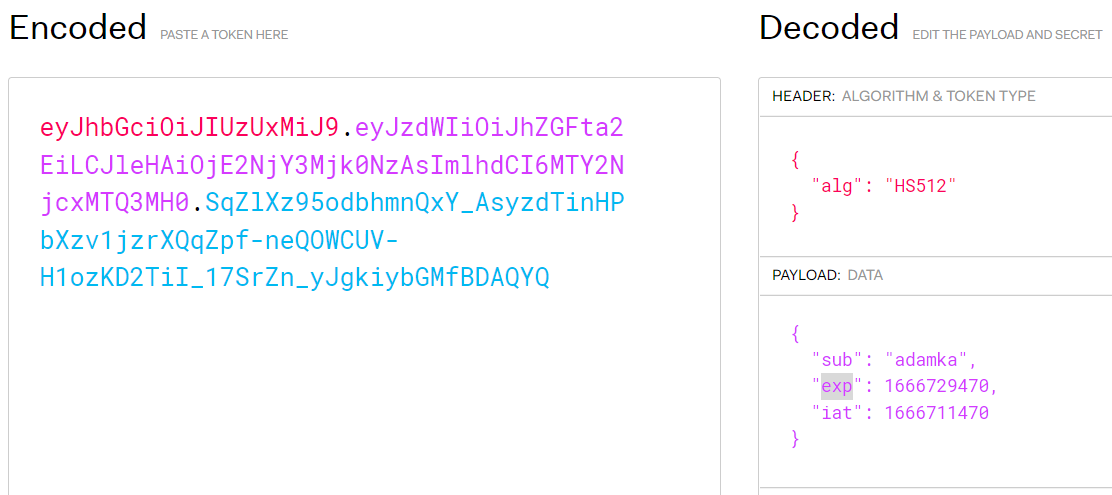
\includegraphics[scale=0.6]{images/jwt.io.png}
\caption{Kódolt és Dekódolt JWT \cite{JWTexample}}
\label{fig:JWT}
\end{figure}